\documentclass{article}
\usepackage[a4paper, total={6.5in, 9in}]{geometry}
\usepackage{amsmath}
\usepackage{graphicx}

\title{Computational Methods: Problem Set 2}
\author{Ian O'Donnell}
\date{\vspace{-5ex}}
\begin{document}
\maketitle
\subsection*{Problem One}
A competitive equilibrium is a set of prices $ \{p_t , r_t, w_t\}_{t=0}^\infty $, an allocation $ \{k_t^d, n_t^d, y_t\}_{t=0}^\infty $
for the firm, and an allocation $ \{c_t, i_t, x_{t+1}, k_t^s, n_t^s,\}_{t=0}^\infty $ for the household such that: 
\begin{enumerate}
    \item The firm's allocation solves: 
    \begin{align*}
        \max_{k_t, n_t} \pi = \sum_{t=0}^{\infty} p_t [y_t - r_t k_t - w_t n_t] \\
        \text{s.t.} \quad y_t \leq F(k_t, n_t)\\
    \end{align*}

    \item The household's allocation solves: 
    \begin{gather*}
        \max_{c_t, n_t, k_{t+1}} \sum_{t=0}^{\infty} \beta^t u(c_t, n_t) \\
        \text{s.t.} \quad \sum_{t=0}^{\infty} p_t[c_t + i_t] \leq \sum_{t=0}^{\infty} p_t[r_t k_t + w_t n_t] + \pi _t \\
        x_{t+1} = (1-\delta) x_t + i_t, \quad 0 \leq n_t \leq 1, \quad 0 \leq k_t \leq x_t \\
        k_0 \quad \text{given}, \quad c_t \geq 0, \quad x_{t+1} \geq 0 \\
        \text{TVC:} \quad \lim_{t \rightarrow \infty} p_t k_{t+1} = 0 
    \end{gather*}

    \item All markets clear for all $t$: $k_t^d = k_t^s$, $n_t^d = n_t^s$, $c_t + i_t = y_t$
\end{enumerate}

\subsection*{Problem 2}
We have that $F(k_t, l_t) = z k_t^\alpha l_t^{1-\alpha}$. 

The first order conditions are: 
\begin{align*}
    \beta^t c_t^{-\sigma} &= \lambda p_t \\
    \beta^t \chi l_t^\eta &= \lambda p_t w_t \\
    \lambda p_t &= \lambda p_{t+1} (1 - \delta + r_{t+1})\\
    z \alpha k_t^{\alpha - 1} l_t^{1-\alpha} - r_t &= 0 \\
    z (1 - \alpha) k_t^{\alpha} l_t^{-\alpha} - w_t &= 0 \\
    \text{Market Clearing:} \quad c_t + [k_{t+1} - (1-\delta)k_t] &= z k_t^\alpha l_t^{1-\alpha} 
\end{align*}

The first and third FOCs, as well as the assumption of steady state gives: 
\begin{equation}
    \bar{r} = \frac{1}{\beta} - 1 + \delta
\end{equation}

The fourth FOC gives:
\begin{equation}
    l_t^{1-\alpha} = \frac{r_t}{z \alpha k_t^{\alpha - 1}} 
\end{equation}

Subbing equation 2 into the market clearing condition, as well as the assumption of steady state, gives: 
\begin{equation}
    \bar{c} = (\frac{\bar{r}}{\alpha} - \delta) \bar{k}
\end{equation}

The first, second and fifth FOCs give: 
\begin{equation}
    c_t^{-\sigma} = \frac{\chi l_t^{\eta+1}}{z(1-\alpha) k_t^\alpha l_t^{1-\alpha}}
\end{equation}

Subbing the second equation into the fourth gives:
\begin{equation}
    \bar{c} = \chi^{\frac{-1}{\sigma}} [r^{\frac{\eta + \alpha}{1-\alpha}}(\frac{1}{z\alpha})^{\frac{1+\eta}{1-\alpha}}
    (\frac{\alpha}{1-\alpha})]^{\frac{-1}{\sigma}} k^{\frac{-\eta}{\sigma}}
\end{equation}

Subbing equation 5 into the market clearing condition gives: 
\begin{equation}
    \bar{k} = [\chi^{\frac{-1}{\sigma}} D^{\frac{-1}{\sigma}}(\frac{\bar{r}}{\alpha}-\delta)^{-1}]^{\frac{\sigma}{\sigma+\eta}}
\end{equation}

Where $D = r^{\frac{\eta + \alpha}{1-\alpha}}(\frac{1}{z\alpha})^{\frac{1+\eta}{1-\alpha}}(\frac{\alpha}{1-\alpha})$

\subsection*{Problem 3}
% Redo to to actually be a dynamic programming problem 
The planners problem is: 

\begin{gather*}
    \max_{c_t, k_t, l_t} \sum_{t=0}^{\infty} \beta^t u(c_t, l_t) \\
    \text{s.t.} \quad F(k_t, l_t) = c_t + k_{t+1} - (1 - \delta) k_t \\
    \quad c_t \geq 0, \quad k_t \geq 0, \quad 0 \leq l_t \leq 1 \quad \forall t \\
    \quad k_0 \quad \text{given} \\
    \quad \text{TVC:} \quad \lim_{t \rightarrow \infty} \beta^t u'(F(k_t, l_t) - k_{t+1})F_k(k_t, l_t)k_t = 0 
\end{gather*}

The bellman equation is: 

\begin{gather*}
    v(k_t) = \max_{k_{t+1}, l_t} \frac{\left( z k_t^\alpha l_t^{1-\alpha} - k_{t+1} + (1-\delta)k_t \right)^{1-\sigma}}{1-\sigma} -\chi \frac{l_t^{1+\eta}}{1+\eta} + \beta [v(k_{t+1})] \\
    \text{s.t.} \quad 0 \leq l_t \leq 1 
\end{gather*}

\subsection*{Problem 4}
I use $\chi = 34$ which gives $\bar{l} = 0.4004$. (I did this by trial and error)

\subsection*{Problem 5}
Part A: 8.18s, 215 iterations \\
\begin{center}
    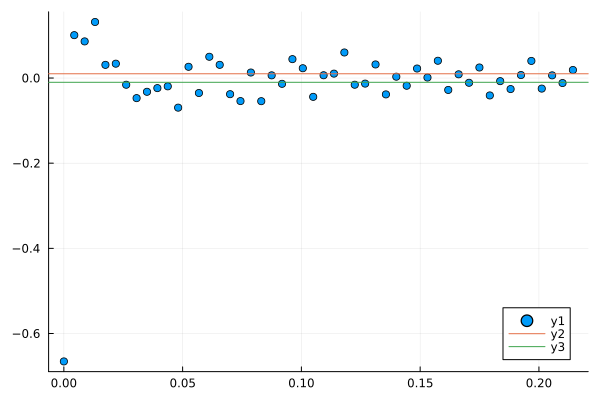
\includegraphics[scale = 0.6]{resid.png}
    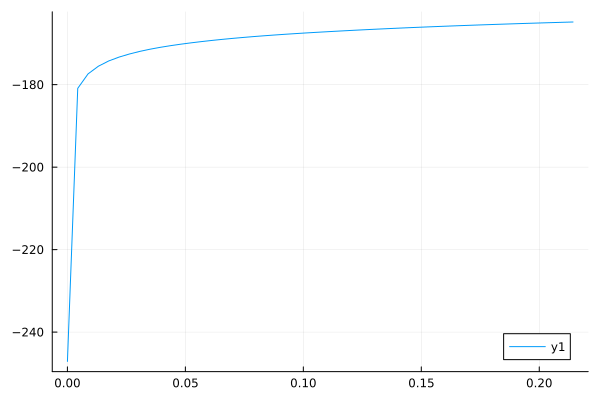
\includegraphics[scale = 0.6]{value.png}
    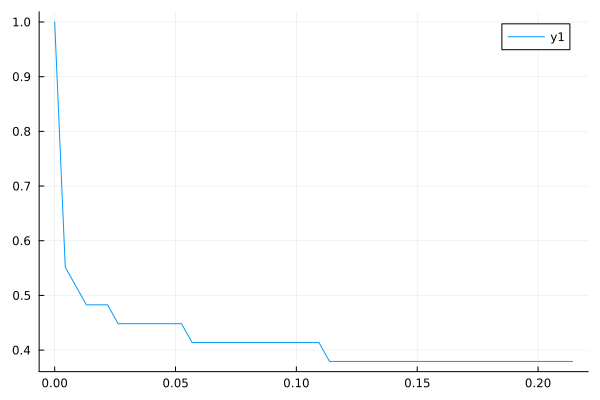
\includegraphics[scale = 0.6]{labour.png}
    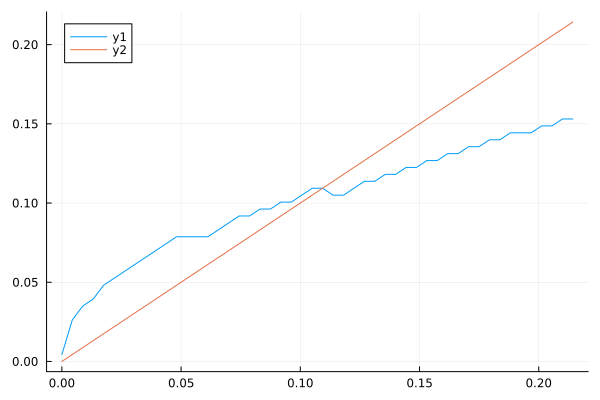
\includegraphics[scale = 0.6]{capital.png}
\end{center}


\end{document}